\documentclass[tikz,convert={outfile=\jobname.svg}]{standalone}
\usepackage{pgf} 
\usepackage{amsmath}
\usepackage{ifthen}
\usetikzlibrary{positioning}
\usetikzlibrary{calc}

\begin{document}
\newcommand{\drawRCC}{
  
\begin{tikzpicture}
    \fill[black] (0,0) rectangle (3, 4);
    \clip (0,0) rectangle (3, 4); 
    \fill[gray] (0, 0.2) arc[start angle=-90, end angle=90, radius=1.8] -- cycle;
    \draw[white, ultra thick] (0, 0.2) arc[start angle=-90, end angle=90, radius=1.8];
    \node[white, anchor=north east, inner sep=2, outer sep=2] at (current bounding box.north east) {RCC};
    \draw[white, ultra thick] (0,0) rectangle (3, 4);
  \end{tikzpicture}
}

\newcommand{\drawMaskedRCC}[4]{
  \pgfmathsetseed{#1}
  \begin{tikzpicture}
    \fill[black] (0,0) rectangle (3, 4);
    \clip (0,0) rectangle (3, 4); 
    \fill[gray] (0, 0.2) arc[start angle=-90, end angle=90, radius=1.8] -- cycle;
    \draw[white, ultra thick] (0, 0.2) arc[start angle=-90, end angle=90, radius=1.8];
    \node[white, anchor=north east] at (3, 4) {RCC};
    \draw[white, ultra thick] (0,0) rectangle (3, 4);
    \foreach \x in {0, 1, 2} {
      \foreach \y in {0, 1, 2, 3} {
        \draw[white, very thin] (\x, \y) rectangle (\x+1, \y+1);
        \pgfmathsetmacro{\rand}{random}
        \ifdim \rand pt < \dimexpr#2 pt\relax
          \fill[#3, opacity=#4] (\x, \y) rectangle (\x+1, \y+1);
        \else
          \fill[black] (\x, \y) rectangle (\x+1, \y+1);
        \fi
      }
    }
  \end{tikzpicture}
}

\newcommand{\drawMLP}{
  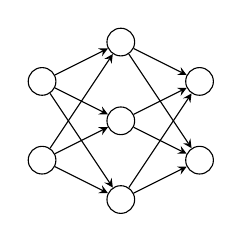
\begin{tikzpicture}
    % Input layer
    \foreach \i in {1, 2} {
      \node[circle, draw=black, fill=white, minimum size=10pt, inner sep=0pt] (input\i) at (0, -\i-0.5) {};
    }

    % Hidden layer
    \foreach \i in {1, 2, 3} {
      \node[circle, draw=black, fill=white, minimum size=10pt, inner sep=0pt] (hidden\i) at (1, -\i) {};
    }

    % Output layer
    \foreach \i in {1, 2} {
      \node[circle, draw=black, fill=white, minimum size=10pt, inner sep=0pt] (output\i) at (2, -\i-0.5) {};
    }

    % Connections from input to hidden layer
    \foreach \i in {1, 2} {
      \foreach \j in {1, 2, 3} {
        \draw[->, black, >=stealth] (input\i) -- (hidden\j);
      }
    }

    % Connections from hidden to output layer
    \foreach \i in {1, 2, 3} {
      \foreach \j in {1, 2} {
        \draw[->, black, >=stealth] (hidden\i) -- (output\j);
      }
    }
  \end{tikzpicture}
}

\newcommand{\drawFeatures}[3]{
  \begin{tikzpicture}
  \pgfmathsetseed{#1}
  \foreach \i in {0, ..., #2} {
    \node at (\i*0.8, 0) {
      $\color{#3}\scriptsize\begin{bmatrix}
        \pgfmathsetmacro{\rand}{rnd*9.9}
        \pgfmathprintnumber[fixed, precision=1]{\rand} \\
        \pgfmathsetmacro{\rand}{rnd*9.9}
        \pgfmathprintnumber[fixed, precision=1]{\rand} \\
        \vdots \\
        \pgfmathsetmacro{\rand}{rnd*9.9}
        \pgfmathprintnumber[fixed, precision=1]{\rand} \\
        \pgfmathsetmacro{\rand}{rnd*9.9}
        \pgfmathprintnumber[fixed, precision=1]{\rand}
      \end{bmatrix}$
    };
  }
  \end{tikzpicture}
}


\newcommand{\drawPosEnc}{
  \begin{tikzpicture}
  \node[circle, draw=black, minimum size=6cm] (circle) at (0, 0) {};
  \draw[black] (-3, 0) sin (-1.5, -1) cos (0, 0) sin (1.5, 1) cos (3, 0);
  \end{tikzpicture}
}
\tikzset{every picture/.style={/utils/exec={\sffamily}}}


\newcommand{\drawRCCPosition}[2]{
  \begin{tikzpicture}
    \node[inner sep=0, outer sep=0, name=rcc] at (0, 0){\drawRCC};
    \ifthenelse{\equal{#1}{x}}{
        \fill[left color=purple, right color=yellow, opacity=0.33] (rcc.south west) rectangle (rcc.north east);
    }{
        \fill[top color=purple, bottom color=yellow, opacity=0.33] (rcc.south west) rectangle (rcc.north east);
    }
    \node[circle, fill=red, inner sep=1pt, name=point1] at (1, 1) {};
    \node[circle, fill=red, inner sep=1pt, name=point2] at (-0.5, -0.5) {};
  \end{tikzpicture}
}

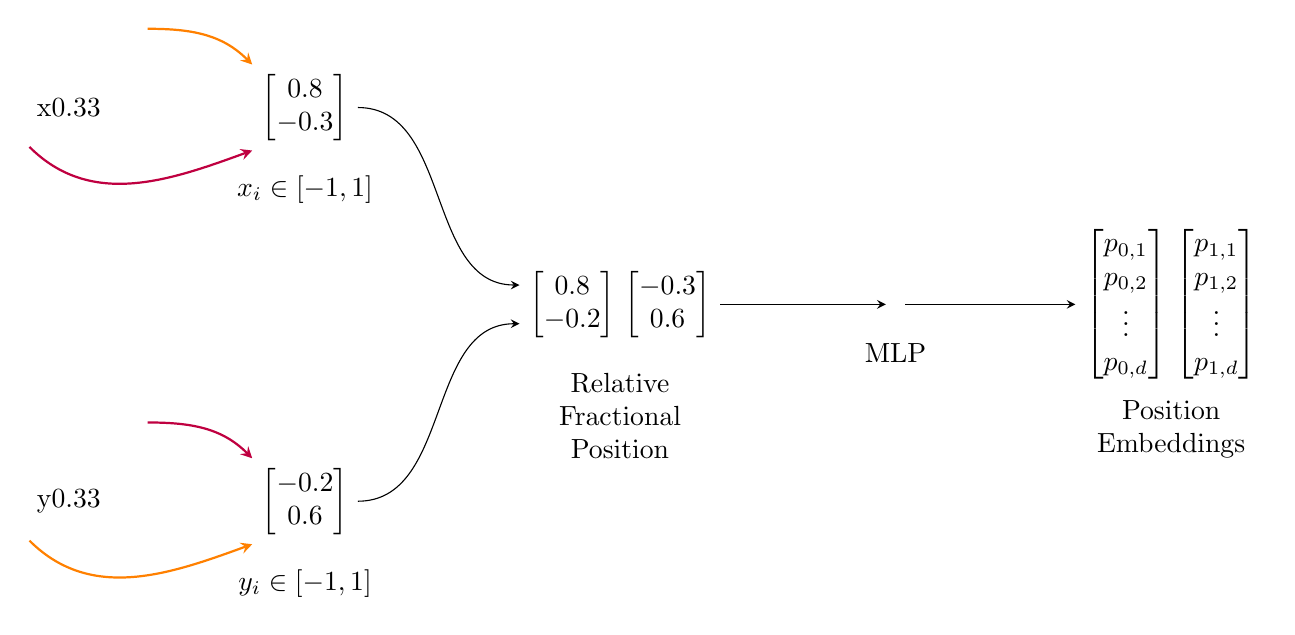
\begin{tikzpicture}
    % Draw RCCs with overlay
    \node[name=rccx] at (0, 0){\drawRCCPosition{x}{0.33}};
    \node[name=rccy] at (0, -5){\drawRCCPosition{y}{0.33}};

    % Vector for x-coordinate
    \node[name=vector1] at (3, 0) {
      $\begin{bmatrix}
        0.8 \\
        -0.3
      \end{bmatrix}$
    };
    \node[below=0.2cm of vector1] {$x_i \in [-1, 1]$};
    \draw[<-, orange, >=stealth, thick] (vector1.north west) to[out=135, in=0] ($(rccx) + (1, 1)$);
    \draw[<-, purple, >=stealth, thick] (vector1.south west) to[out=200, in=-45] ($(rccx) + (-0.5, -0.5)$);
    
    % Vector for y-coordinate
    \node[name=vector2] at (3, -5) {
      $\begin{bmatrix}
        -0.2 \\
        0.6 
      \end{bmatrix}$
    };
    \node[below=0.2cm of vector2] {$y_i \in [-1, 1]$};
    \draw[<-, purple, >=stealth, thick] (vector2.north west) to[out=135, in=0] ($(rccy) + (1, 1)$);
    \draw[<-, orange, >=stealth, thick] (vector2.south west) to[out=200, in=-45] ($(rccy) + (-0.5, -0.5)$);

    % Vector for combined coordinate
    \node[name=pos_in] at (7, -2.5) {
      $\begin{bmatrix}
        0.8 \\
        -0.2 
      \end{bmatrix}$
      $\begin{bmatrix}
        -0.3 \\
        0.6
      \end{bmatrix}$
    };
    \node[below=0.2cm of pos_in, align=center] {Relative\\Fractional\\Position};
    \draw[->, black, >=stealth] (vector1.east) to[out=0, in=180] ($(pos_in.north west) + (0, -0.3)$);
    \draw[->, black, >=stealth] (vector2.east) to[out=0, in=180] ($(pos_in.south west) + (0, 0.3)$);

    % MLP
    \node[name=mlp] at (10.5, -2.5){\drawMLP};
    \node[below=0.5cm of mlp.south, anchor=center] {MLP};
    \draw[->, black, >=stealth] (pos_in) -- (mlp);

    % Position embeddings
    \node[name=posemb] at (14, -2.5) {
      $\begin{bmatrix}
        p_{0, 1} \\
        p_{0, 2} \\
        \vdots \\
        p_{0, d}
      \end{bmatrix}$
      $\begin{bmatrix}
        p_{1, 1} \\
        p_{1, 2} \\
        \vdots \\
        p_{1, d}
      \end{bmatrix}$
    };
    \node[below=0.5cm of posemb.south, anchor=center, align=center] {Position\\Embeddings};
    \draw[->, black, >=stealth] (mlp) -- (posemb);

\end{tikzpicture}
\end{document}